\documentclass{article}
\usepackage{amsmath, amssymb}
\usepackage{geometry}
\geometry{margin=1in}
\usepackage{graphicx}
\usepackage{float}
\usepackage{hyperref}

\title{ECON 425: Macroeconomic Policy\\\large Homework Five\\Topic: Optimal Price Setting and Phillips Curves}
\author{Charles Ancel}
\date{\today}

\begin{document}

\maketitle

\section{Introduction}

This homework focuses on optimal price setting in a macroeconomic context and the analysis of Phillips Curves. The solutions provided will demonstrate the application of economic theories and the use of empirical data to validate these theories.

\noindent\rule{\linewidth}{1pt}

\section{Questions and Solutions}

\subsection*{1. Optimal Price Setting}

\subsubsection*{1.1 Substitute the nominal profits in the general problem}

The nominal profits of the firm are given by:
\[
\Pi_{i,t} = Q_{i,t} P_{i,t} - W_t L_{i,t}
\]
Using \(Q_{i,t} = Y_{i,t}\), we get:
\[
\Pi_{i,t} = Y_{i,t} P_{i,t} - W_t L_{i,t}
\]

Substituting into the general problem:
\[
\max \sum_{k=0}^{\infty} \beta_F^k \frac{\Pi_{i,t+k}}{P_{t+k}}
\]
\[
\max \sum_{k=0}^{\infty} \beta_F^k \left( \frac{Y_{i,t+k} P_{i,t+k} - W_{t+k} L_{i,t+k}}{P_{t+k}} \right)
\]

Using equations 3.1 and 3.2:
\[
Y_{i,t} = Y_t \left( \frac{P_{i,t}}{P_t} \right)^{-\eta}
\]
\[
\max_{ \{P_{i,t}\}_{t=0}^{\infty} } \sum_{k=0}^{\infty} \beta_F^k \left[ Y_{t+k} \left( \frac{P_{i,t+k}}{P_{t+k}} \right)^{-\eta} P_{i,t+k} - W_{t+k} L_{i,t+k} \right]
\]

\noindent\rule{\linewidth}{0.5pt}

\subsubsection*{1.2 Take the partial derivative of the objective function with respect to \( P_{i,t} \), and solve for the optimal price \( P_{i,t}^* \)}

Taking the partial derivative with respect to \( P_{i,t} \):
\[
\frac{\partial}{\partial P_{i,t}} \sum_{k=0}^{\infty} \beta_F^k \left[ \frac{Y_{t+k} \left( \frac{P_{i,t+k}}{P_{t+k}} \right)^{-\eta} P_{i,t+k} - W_{t+k} L_{i,t+k}}{P_{t+k}} \right]
\]
\[
= \sum_{k=0}^{\infty} \beta_F^k \left[ -\eta Y_{t+k} \left( \frac{P_{i,t+k}}{P_{t+k}} \right)^{-\eta-1} \frac{P_{i,t+k}}{P_{t+k}} + Y_{t+k} \left( \frac{P_{i,t+k}}{P_{t+k}} \right)^{-\eta} \frac{1}{P_{t+k}} \right]
\]

Setting this derivative to zero for maximization:
\[
-\eta Y_t \left( \frac{P_{i,t}}{P_t} \right)^{-\eta-1} \frac{P_{i,t}}{P_t} + Y_t \left( \frac{P_{i,t}}{P_t} \right)^{-\eta} \frac{1}{P_t} = 0
\]

Solving for \( P_{i,t} \):
\[
P_{i,t}^* = \frac{\eta}{\eta-1} W_t
\]

\noindent\rule{\linewidth}{0.5pt}

\subsubsection*{1.3 Repeat the previous step for the prices of periods \( t+1 \) and \( t+2 \)}

For \( t+1 \):
\[
P_{i,t+1}^* = \frac{\eta}{\eta-1} W_{t+1}
\]

For \( t+2 \):
\[
P_{i,t+2}^* = \frac{\eta}{\eta-1} W_{t+2}
\]

\noindent\rule{\linewidth}{0.5pt}

\subsubsection*{1.4 Express the whole set of optimal prices synthetically}

The general form for the optimal price \( P_{i,t+k}^* \) can be expressed as:
\[
P_{i,t+k}^* = \frac{\eta}{\eta-1} W_{t+k}
\]

\noindent\rule{\linewidth}{1pt}

\subsection*{2. Phillips Curves and AS Curves}

\subsubsection*{2.1 Explanation of Figure 1 in Phillips (1958)}

In the first few pages of Phillips (1958), the relationship between unemployment and the rate of change of money wage rates in the United Kingdom is examined. Figure 1 shows a scatter plot with a downward-sloping curve, indicating that higher unemployment rates are associated with lower rates of wage inflation. This curve suggests an inverse relationship between unemployment and wage inflation.

\noindent\rule{\linewidth}{0.5pt}

\subsubsection*{2.2 Explanation and comparison of Figures in Samuelson and Solow (1960) with Phillips (1958)}

In Samuelson and Solow (1960), Figure 2 illustrates the trade-off between unemployment and inflation based on their empirical analysis. Compared to Figure 1 in the same paper, which depicts a similar inverse relationship between wage inflation and unemployment, Figure 2 incorporates a broader analysis of inflation.

Comparing these figures with Figure 1 in Phillips (1958), Samuelson and Solow's figures extend the analysis to general inflation, not just wage inflation. The key difference is that Phillips focused on wage inflation, while Samuelson and Solow looked at overall inflation, making their analysis more relevant for general economic policy.

\noindent\rule{\linewidth}{0.5pt}

\subsubsection*{2.3 Data Analysis from FRED}

The following R code retrieves the required data from FRED, calculates inflation and wage inflation rates, merges the data, and plots the relationships:

\begin{verbatim}
library(tidyverse)
library(quantmod)
library(fredr)

fredr_set_key("89e09406a6b0e5d39d06d3b19fec5156")

unemployment_rate <- fredr(series_id = "UNRATE")
cpi <- fredr(series_id = "CPILFESL")
hourly_earnings <- fredr(series_id = "CES0500000003")

unemployment_ts <- xts(unemployment_rate$value, order.by = as.Date(unemployment_rate$date))
cpi_ts <- xts(cpi$value, order.by = as.Date(cpi$date))
earnings_ts <- xts(hourly_earnings$value, order.by = as.Date(hourly_earnings$date))

inflation_rate <- diff(log(cpi_ts), lag = 12) * 100
wage_inflation_rate <- diff(log(earnings_ts), lag = 12) * 100

data <- merge(unemployment_ts, inflation_rate, wage_inflation_rate, all = FALSE)
colnames(data) <- c("Unemployment_Rate", "Inflation_Rate", "Wage_Inflation_Rate")

data_df <- data.frame(date = index(data), coredata(data))

# Plot Inflation vs. Unemployment Rate
ggplot(data_df, aes(x = Unemployment_Rate, y = Inflation_Rate)) +
  geom_point() +
  geom_smooth(method = "lm") +
  labs(title = "Inflation vs. Unemployment Rate",
       x = "Unemployment Rate (%)",
       y = "Inflation Rate (%)")

# Plot Wage Inflation vs. Unemployment Rate
ggplot(data_df, aes(x = Unemployment_Rate, y = Wage_Inflation_Rate)) +
  geom_point() +
  geom_smooth(method = "lm") +
  labs(title = "Wage Inflation vs. Unemployment Rate",
       x = "Unemployment Rate (%)",
       y = "Wage Inflation Rate (%)")

# Analyze the relationship between variables
model1 <- lm(Inflation_Rate ~ Unemployment_Rate, data = data_df)
summary(model1)

model2 <- lm(Wage_Inflation_Rate ~ Unemployment_Rate, data = data_df)
summary(model2)
\end{verbatim}
The following figures show the relationship between the unemployment rate and both the inflation rate and wage inflation rate.

\begin{figure}[H]
    \centering
    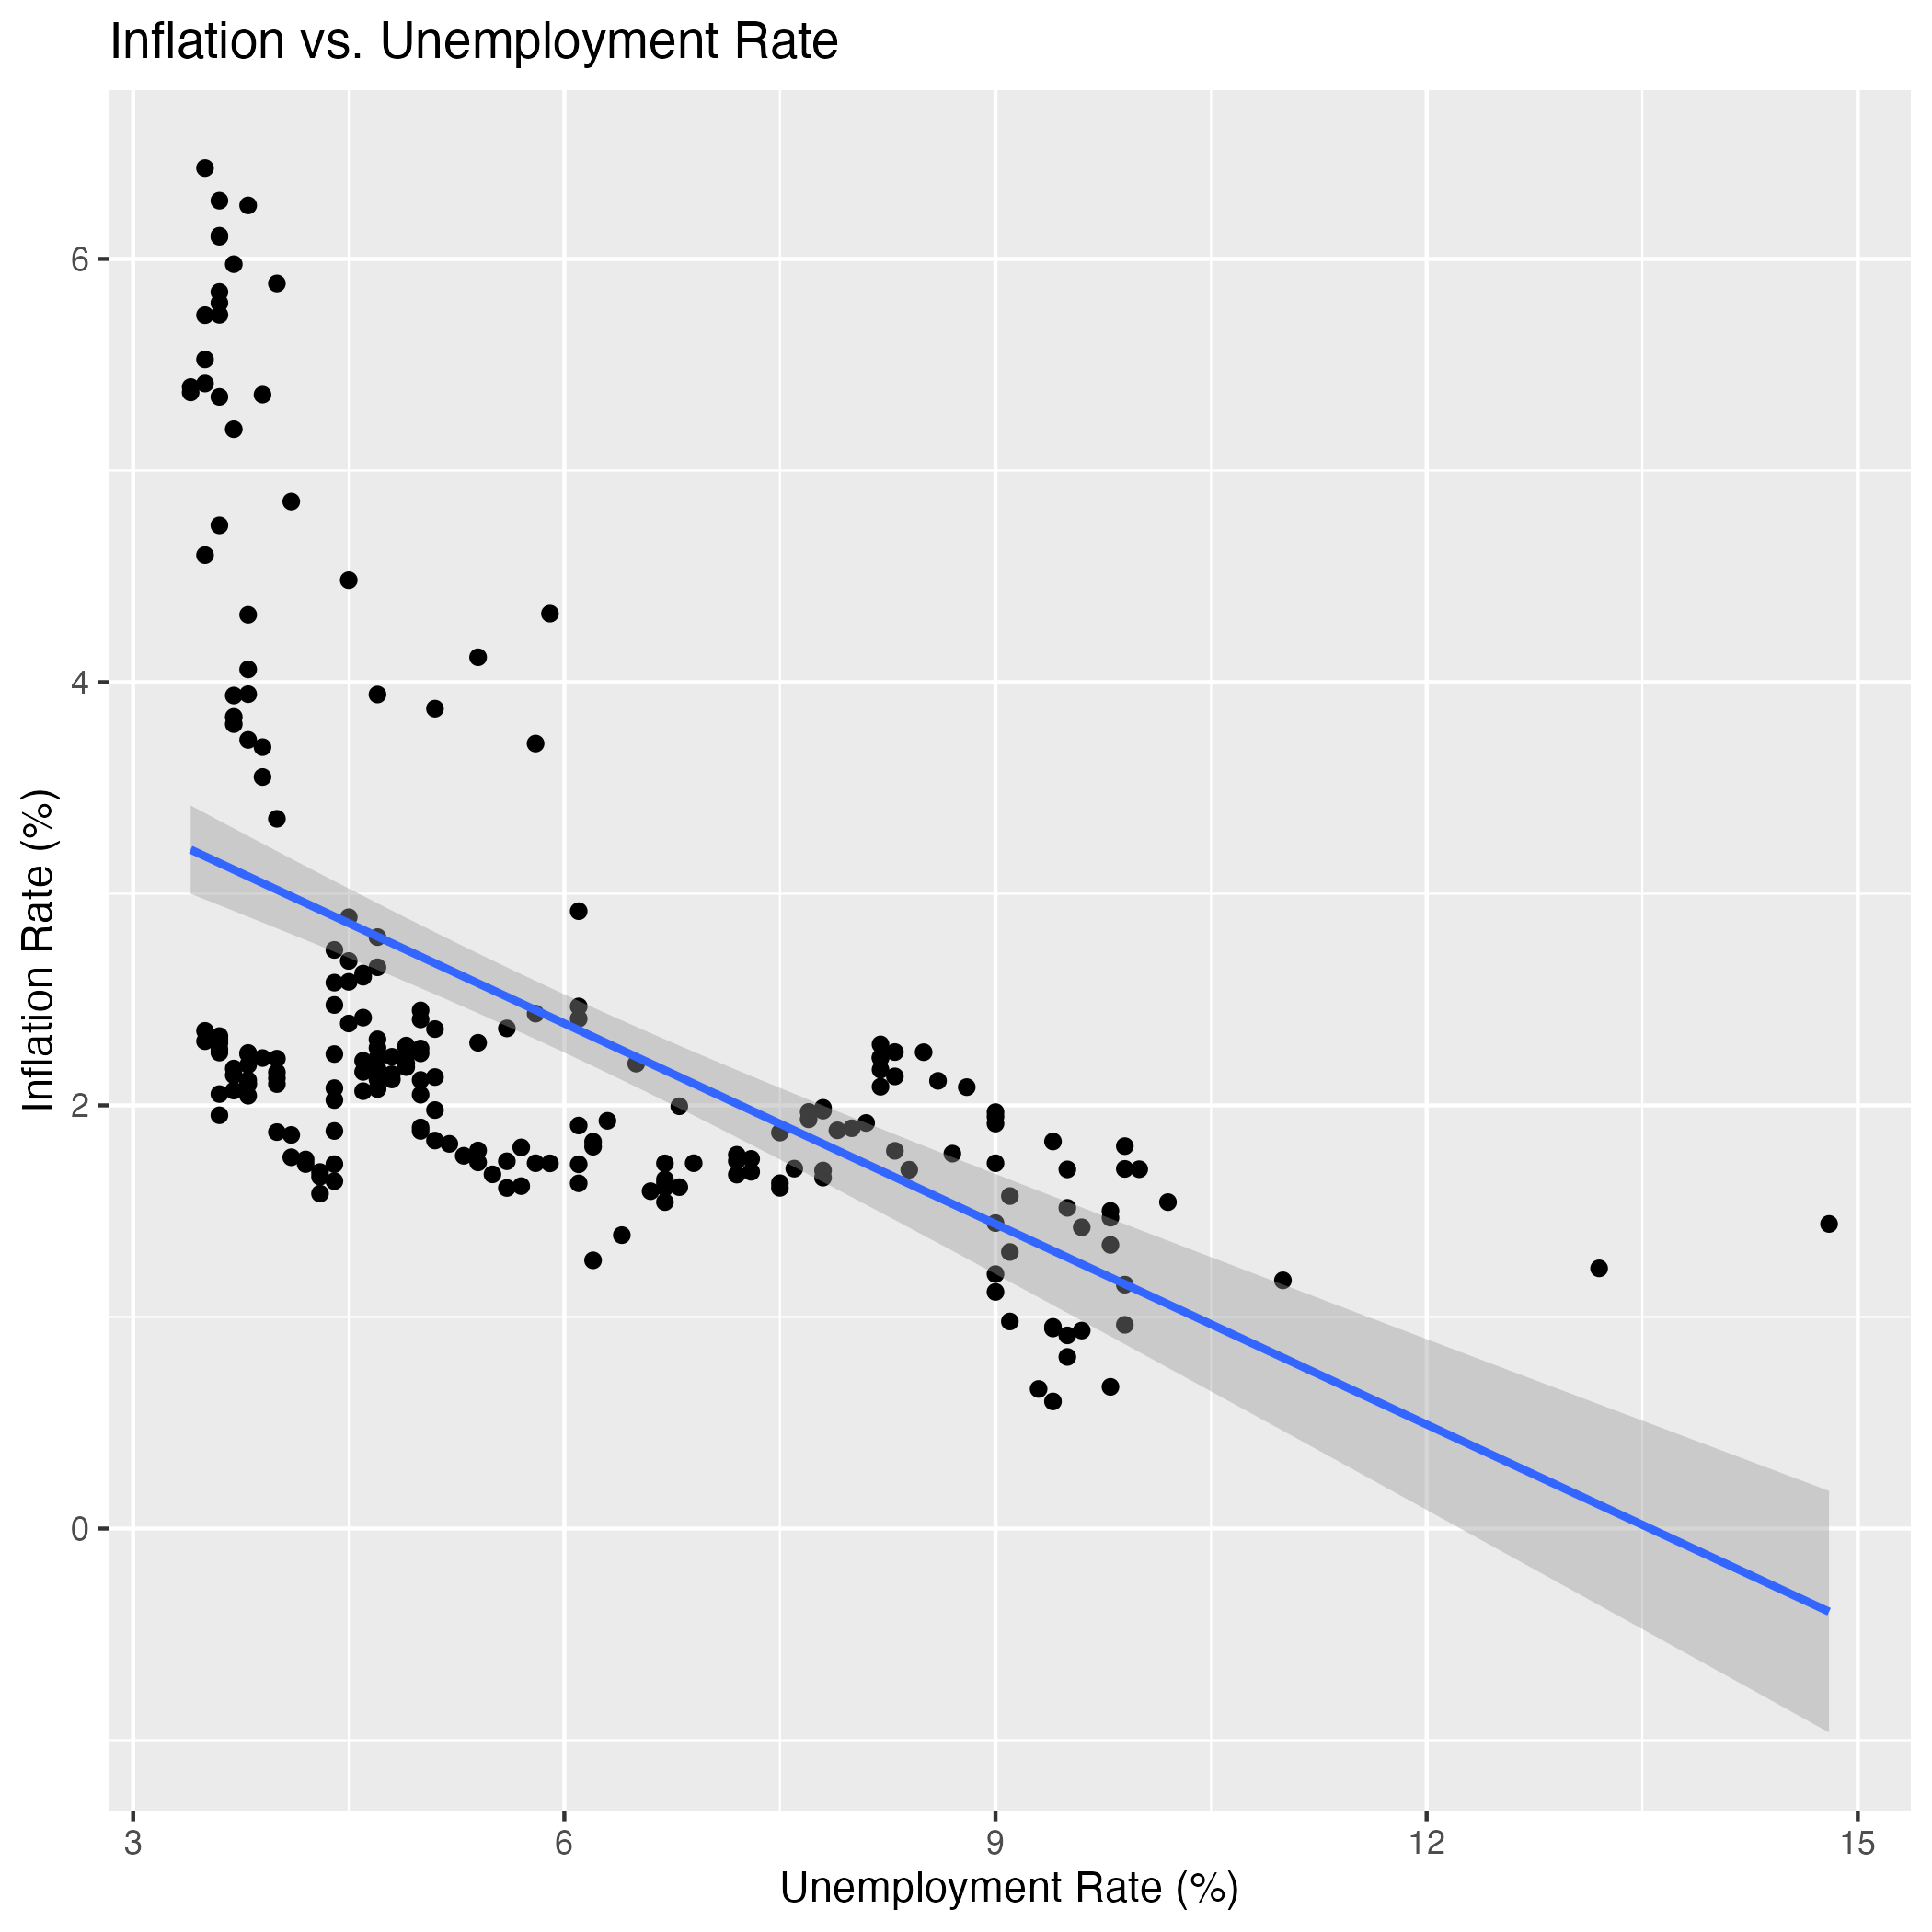
\includegraphics[width=0.8\textwidth]{/Users/cancel/Personal/Coursework/Econ425/HW5/R/Inflation_vs_Unemployment.png}
    \caption{Inflation vs. Unemployment Rate}
\end{figure}

\begin{figure}[H]
    \centering
    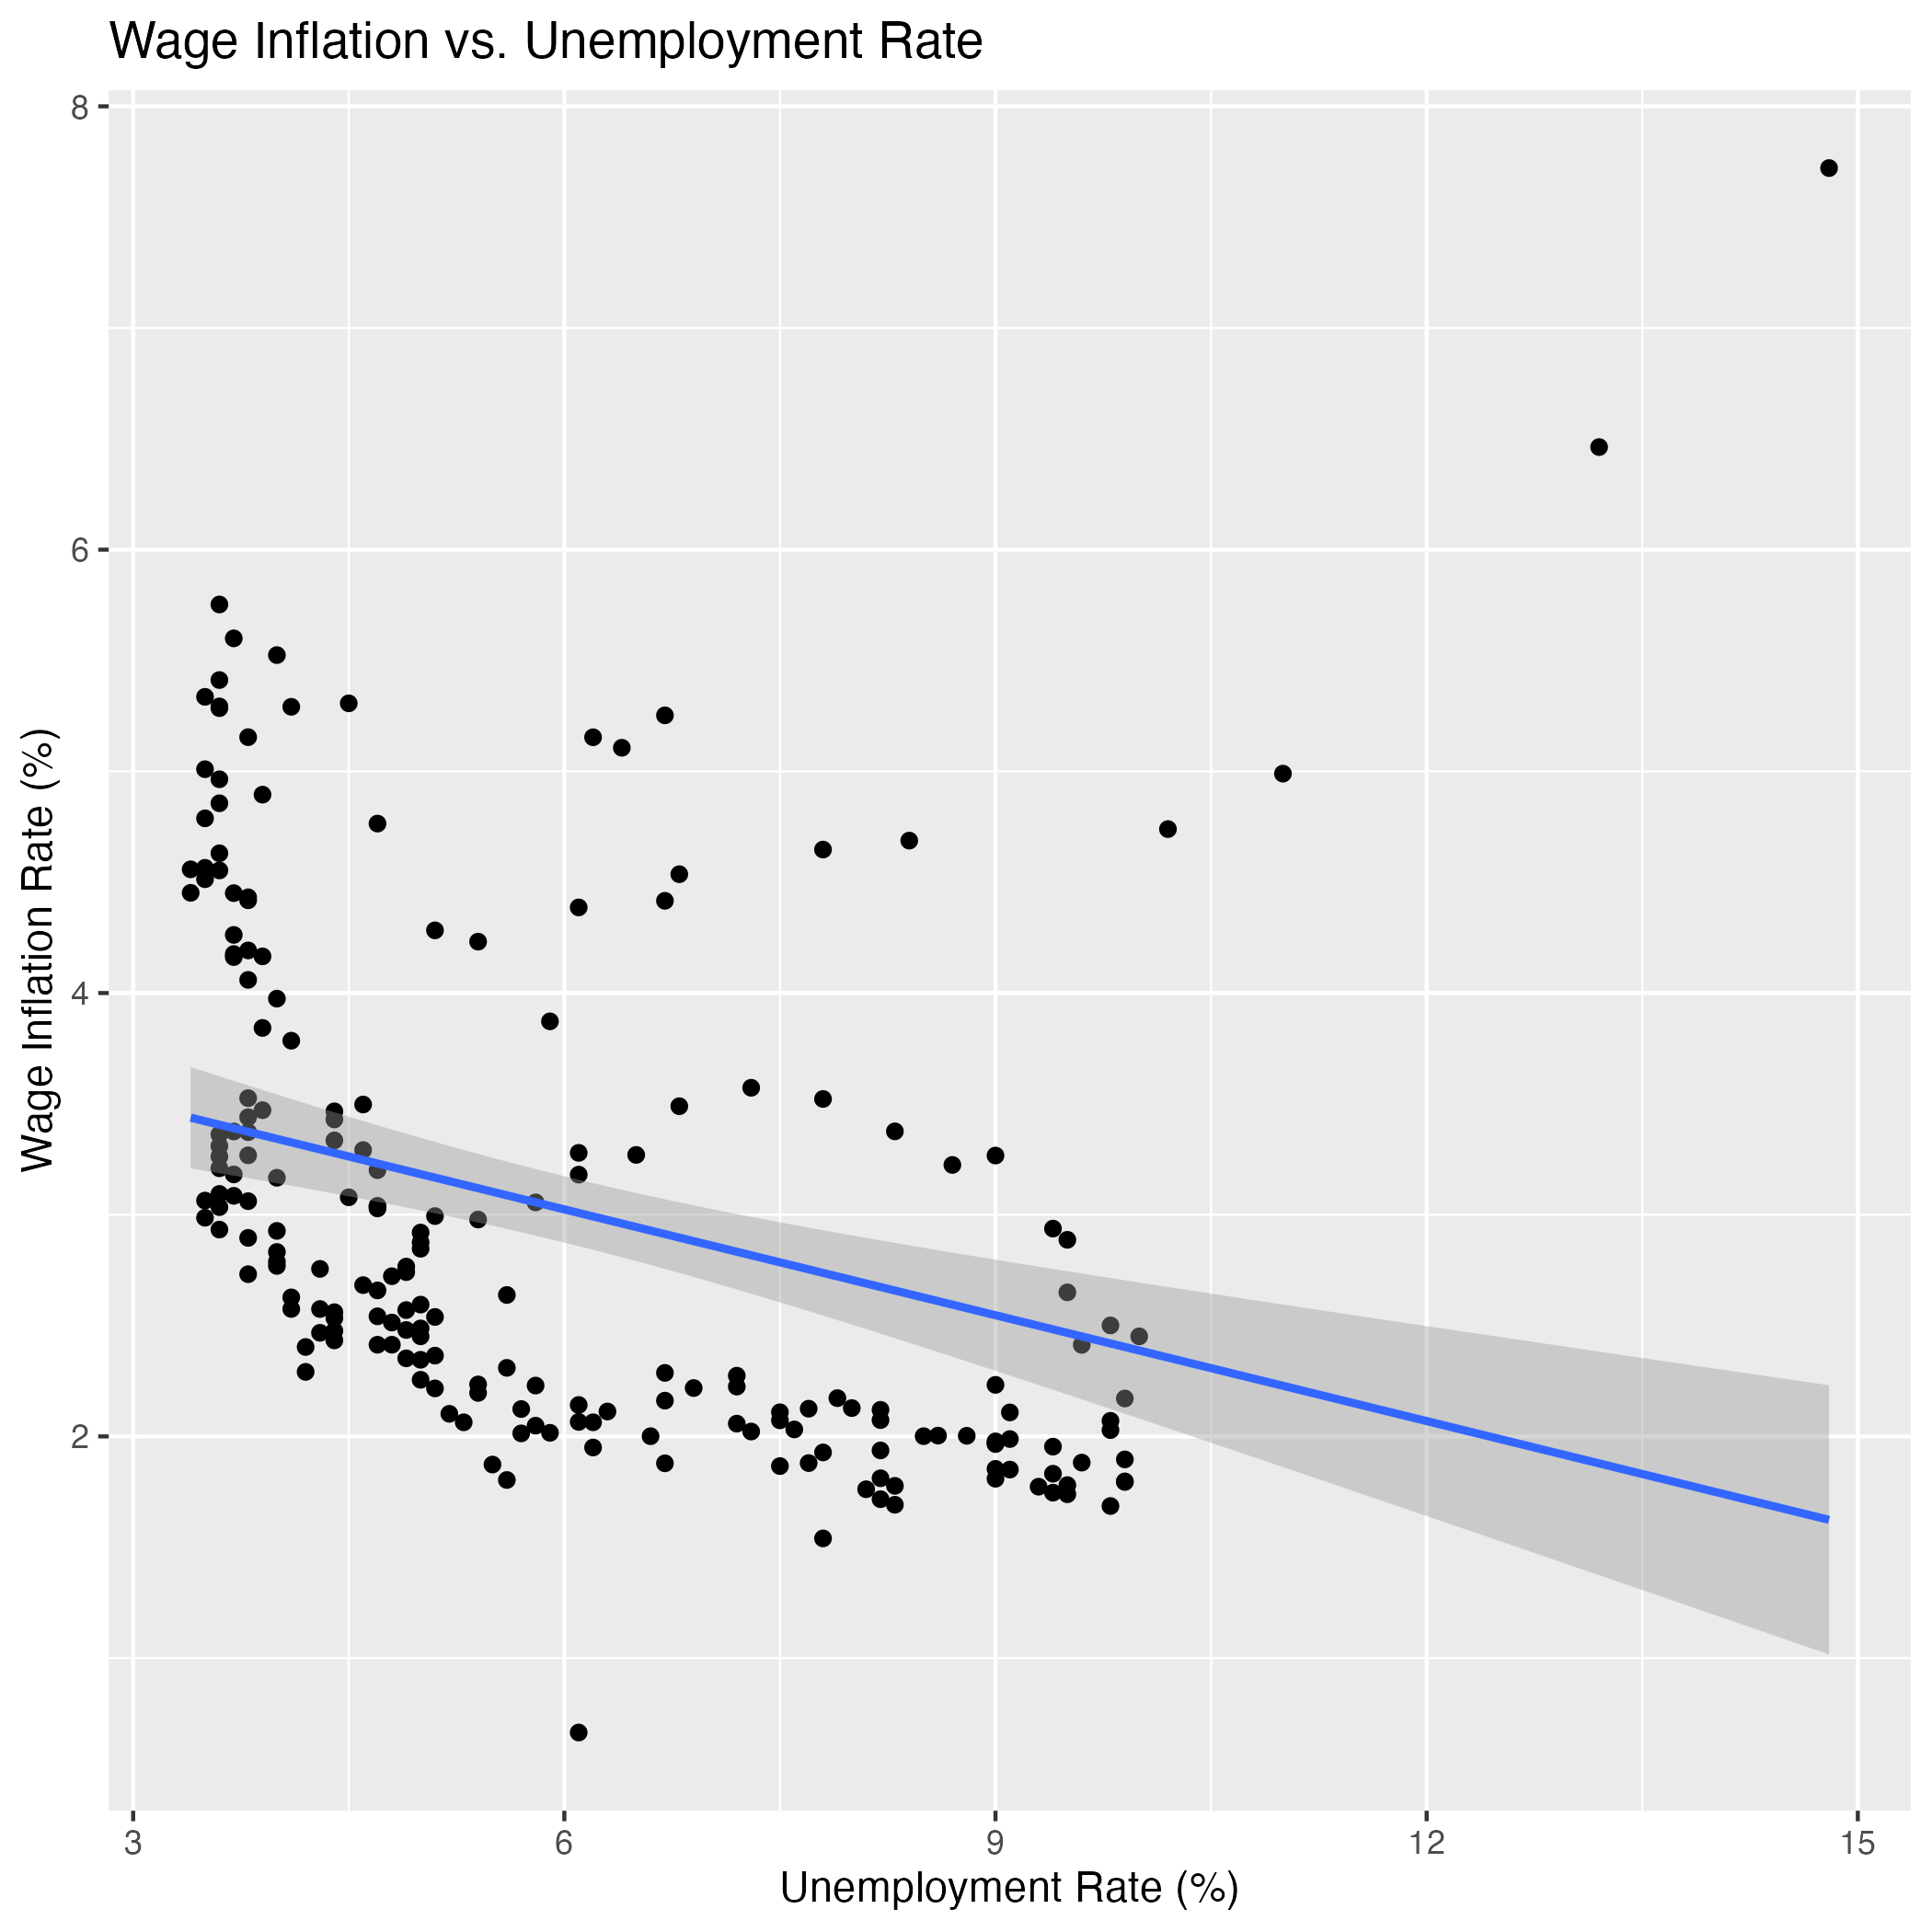
\includegraphics[width=0.8\textwidth]{/Users/cancel/Personal/Coursework/Econ425/HW5/R/Wage_Inflation_vs_Unemployment.png}
    \caption{Wage Inflation vs. Unemployment Rate}
\end{figure}

\noindent\rule{\linewidth}{0.5pt}

\subsubsection*{2.4 Discussion on Challe's AS Curve and the Phillips Curve}

Challe refers to the AS curve as "A Phillips Curve" because the AS (Aggregate Supply) curve incorporates the relationship between inflation and economic activity, similar to the Phillips Curve, which shows the inverse relationship between unemployment and inflation. Both curves highlight the trade-off between inflation and economic variables like unemployment or output.

\noindent\rule{\linewidth}{1pt}

\subsection*{3 Exercise 3.7.1: Price Indexation to Trend Inflation}

Given the AS curve:
\[
\pi_t = \phi \pi_{t-1} + (1-\phi) \bar{\pi} + \kappa (Y_t - Y_t^n)
\]

Incorporate the fraction \( \phi \) indexing to past inflation and the rest indexing to trend inflation. This modification changes the AS curve to:
\[
\pi_t = \phi \pi_{t-1} + (1-\phi) \pi^T + \kappa (Y_t - Y_t^n)
\]
where \( \pi^T \) is the trend inflation.

\noindent\rule{\linewidth}{0.5pt}

\subsubsection*{3.1 Consistency with the Natural Rate Hypothesis}

The natural rate hypothesis asserts that inflation will eventually return to its expected level regardless of current economic conditions. The modified AS curve incorporates both past inflation and trend inflation, suggesting that while short-term deviations may occur, inflation expectations (trend inflation) still play a crucial role, aligning with the natural rate hypothesis.

\noindent\rule{\linewidth}{0.5pt}

\subsubsection*{3.2 Consistency with Blanchard's Evidence}

Blanchard's analysis suggests that inflation dynamics have become more anchored, with inflation expectations playing a significant role. The modified AS curve, which includes trend inflation, is consistent with this view as it reflects the importance of inflation expectations in determining actual inflation.

\noindent\rule{\linewidth}{1pt}

\end{document}
